\chapter{Dronetag backend infrastructure}\label{ch:dronetag-backend-infrastructure}
This chapter describes all Dronetag backend infrastructure and contains a detailed description of the web Droneteg platform.
It consists the whole technical stack that ensures data providing.
My co-workers had to determine the convenient and reliable way how to gradually construct a useful architecture of the infrastructure.
It starts with an IoT module and simplified web, and it continues to implement WebSockets with alone Live Service.
Current parts of the stack is following:
\begin{itemize}
    \item Backend,
    \item Frontend,
    \item OLP Message Broker,
    \item Live Service and
    \item .
\end{itemize}
Every web application in stack is deployed and managed by Docker. %\cite{}
It is the easiest way to develop and publish new version software.
Thanks to docker compose tool we can have a separated parts of the infrastructure.
In case of bigger changes, we have to change only one and others are without changes.

Due to security reasons, the web API is divided to Private and Public API endpoints.

In additional determination, this infrastructure is divided to Staging and Production environment.
Staging is for development and testing purposes and it usually runs on the same version as Production.
The exception is only when a new feature is establishing.

\section{Backend application}\label{sec:backend-application}
Python Django Web API app %TODO


\section{Database model}\label{sec:database-model}
There is a database model figure in Dronetag backend.
The database model consists followings entities:
\begin{itemize}
    \item User,
    \item Aircraft,
    \item Device,
    \item Flight,
    \item Telemetry measurement,
    \item Organization,
    \item Fleet,
    \item Aircraft vendor,
    \item Aircraft model,
    \item Airspace zone,
    \item User preference and
    \item Organization preference.
\end{itemize}
A detailed diagram with relationships between entities is in the ERD Diagram of infrastructure in this picture.%\cite{fig:erd-diagram}

\subsection{User}\label{subsec:user}
This entity represents a user who signs up and logs in to the application.
...

All attributes are described like this:
\begin{itemize}
    \item id - represents the unique object identificator,
    \item email - represents ...
    \item full\_name - represents
    \item password\_hash - represents
    \item phone\_number - represents
    \item deleted - represents
    \item date\_created - represents
    \item data\_modified - represents
    \item last\_login - represents
    \item active - represents
    \item country - represents
\end{itemize}

\subsection{Aircraft}\label{subsec:aircraft}
This entity represents an aircraft that is connect with a Dronetag device.
...

All attributes are described like this:
\begin{itemize}
    \item id - represents the unique object identificator,
    \item name - represents an aircraft name for easier recognition in My aircraft list,
    \item uas\_operator\_id - represents a unique code identifying a pilot who registered this aircraft,
    \item weight - represents a weight of the aircraft,
    \item date\_created - represents a date when was an aircraft added,
    \item data\_modified - represents a date when was an aircraft changed,
    \item deleted - represents a date when was an aircraft deleted.
\end{itemize}

\subsection{Device}\label{subsec:device}
This entity represents a physical device that sends live information to the Dronetag platform.
...

All attributes are described like this:
\begin{itemize}
    \item id - represents the unique object identificator,
    \item serial\_number - represents ...
    \item name - represents
    \item type - represents
    \item comm\_id - represents
    \item date\_created - represents
    \item date\_modified - represents
    \item last\_battery - represents
    \item last\_rsrp - represents
    \item last\_message - represents
\end{itemize}

\subsection{Flight}\label{subsec:flight}
This entity represents it represents a flight that a user has created.
...

All attributes are described like this:
\begin{itemize}
    \item id - represents the unique object identificator,
    \item date\_planned\_start - represents ...
    \item date\_planned\_finish - represents ...
    \item date\_started - represents ...
    \item date\_finished - represents ...
    \item status - represents
    \item distance - represents
    \item duration - represents
    \item region\_geojson - represents
    \item max\_flight\_altitude - represents
    \item takeoff\_latitude - represents
    \item takeoff\_longitude - represents
    \item takeoff\_geo\_alt - represents
    \item takeoff\_pressure - represents
    \item public - represents
    \item date\_created - represents
    \item date\_modified - represents
    \item deleted - represents
\end{itemize}

\subsection{Telemetry measurement}\label{subsec:telemetry-measurement}
This entity represents a ...

All attributes are described like this:
\begin{itemize}
    \item time\_received - represents the unique object identificator,
    \item time - represents ...
    \item latitude - represents
    \item longitude - represents
    \item altitude - represents
    \item geo\_altitude - represents
    \item velocity\_x - represents
    \item velocity\_y - represents
    \item velocity\_z - represents
    \item gnss\_accuracy - represents
\end{itemize}

\subsection{Organization}\label{subsec:organization}
This entity represents a ...

All attributes are described like this:
\begin{itemize}
    \item id - represents the unique object identificator,
    \item name - represents ...
    \item description - represents
    \item date\_created - represents
    \item date\_modified - represents
    \item deleted - represents
\end{itemize}

\subsection{Fleet}\label{subsec:fleet}
This entity represents a ...

All attributes are described like this:
\begin{itemize}
    \item id - represents the unique object identificator,
    \item name - represents ...
    \item color - represents
    \item deleted - represents
    \item date\_created - represents
    \item date\_modified - represents
\end{itemize}

\subsection{Aircraft vendor}\label{subsec:aircraft-vendor}
This entity represents a ...

All attributes are described like this:
\begin{itemize}
    \item id - represents the unique object identificator,
    \item name - represents a vendor name.
\end{itemize}

\subsection{Aircraft model}\label{subsec:aircraft-model}
This entity represents a user who signs up and logs in to the application.
...

All attributes are described like this:
\begin{itemize}
    \item id - represents the unique object identificator,
    \item name - represents ...
    \item weight - represents
    \item vendor\_id - represents a relationship to a Vendor.
\end{itemize}

\subsection{Airspace zone}\label{subsec:airspace-zone}
This entity represents a ...

All attributes are described like this:
\begin{itemize}
    \item id - represents the unique object identificator,
    \item name - represents ...
    \item country - represents
    \item region\_geojson - represents
    \item date\_created - represents
    \item date\_modified - represents
\end{itemize}

\subsection{User preference}\label{subsec:user-preference}
This entity represents a ...

All attributes are described like this:
\begin{itemize}
    \item property - represents ...
    \item value - represents ...
    \item date\_modified - represents
\end{itemize}

\subsection{Organization preference}\label{subsec:organization-preference}
This entity represents a user who signs up and logs in to the application.
...

All attributes are described like this:
\begin{itemize}
    \item property - represents the unique object identificator,
    \item value - represents ...
    \item date\_modified - represents
\end{itemize}

\begin{figure}
    \centering
    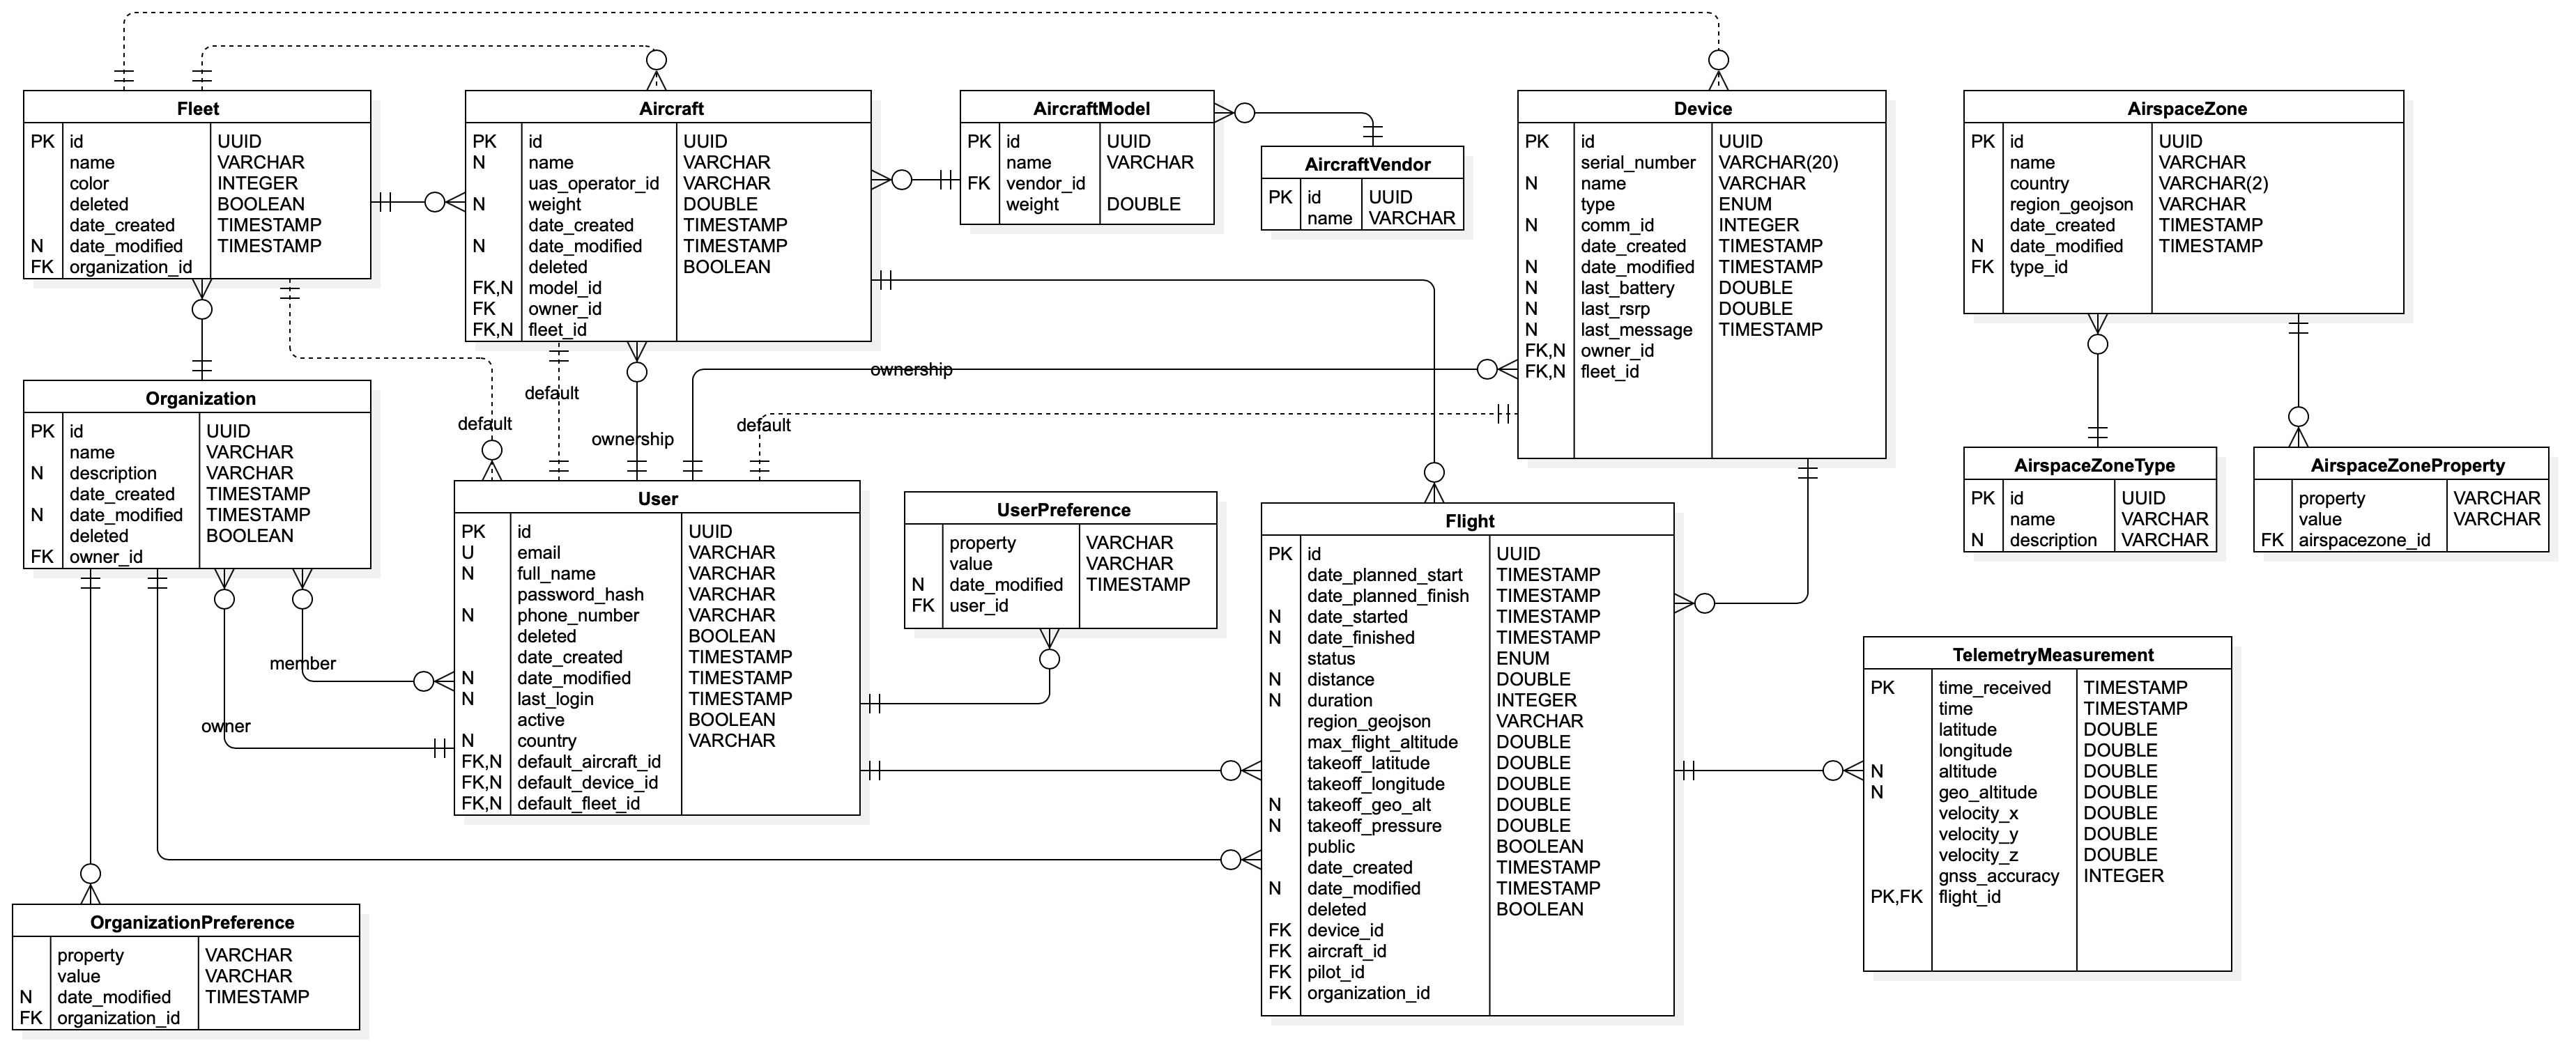
\includegraphics[scale=0.31, angle=90]{assets/erd_diagram.png}
    \caption{ERD Diagram of data model\cite{dataModel}}
    \label{fig:erd-diagram}
\end{figure}

\subsection{Live Service database model}\label{subsec:live-service-database-model}
In additional, during the development we had found out the current backend is not sufficient for our needs, so we decided to divide the backend model into backend one and Live Service model.
Because there are only live real time temporary data, so we deployed a Redis database.

"Redis is an open source (BSD licensed), in-memory data structure store, used as a database, cache and message broker.
It supports data structures such as strings, hashes, lists, sets, sorted sets with range queries, bitmaps, hyperloglogs, geospatial indexes with radius queries and streams.
Redis has built-in replication, Lua scripting, LRU eviction, transactions and different levels of on-disk persistence, and provides high availability via Redis Sentinel and automatic partitioning with Redis Cluster."\cite{redis}
It means that the Redis is a real-time storage that persists data only for very short time.
That is the reason, why it is suitable for this purpose.

The Live Service database model consists of \textbf{Device} and \textbf{Telemetry} entity.



\section {Broker}\label{sec:broker}

